\documentclass[a4paper,12pt,times,numbered,print,index]{Classes/PhDThesisPSnPDF}

% ********************************** Preamble **********************************
% Preamble: Contains packages and user-defined commands and settings
% ******************************************************************************
% ****************************** Custom Language *********************************
\usepackage[italian]{babel}


% ******************************************************************************
% ****************************** Custom Margin *********************************

% Add `custommargin' in the document class options to use this section
% Set {innerside margin / outerside margin / topmargin / bottom margin}  and
% other page dimensions
\ifsetCustomMargin
  \RequirePackage[left=37mm,right=30mm,top=35mm,bottom=30mm]{geometry}
  \setFancyHdr % To apply fancy header after geometry package is loaded
\fi

% Add spaces between paragraphs
%\setlength{\parskip}{0.5em}
% Ragged bottom avoids extra whitespaces between paragraphs
\raggedbottom
% To remove the excess top spacing for enumeration, list and description
%\usepackage{enumitem}
%\setlist[enumerate,itemize,description]{topsep=0em}

% *****************************************************************************
% ******************* Fonts (like different typewriter fonts etc.)*************

% Add `customfont' in the document class option to use this section

\ifsetCustomFont
  % Set your custom font here and use `customfont' in options. Leave empty to
  % load computer modern font (default LaTeX font).
  %\RequirePackage{helvet}

  % For use with XeLaTeX
  %  \setmainfont[
  %    Path              = ./libertine/opentype/,
  %    Extension         = .otf,
  %    UprightFont = LinLibertine_R,
  %    BoldFont = LinLibertine_RZ, % Linux Libertine O Regular Semibold
  %    ItalicFont = LinLibertine_RI,
  %    BoldItalicFont = LinLibertine_RZI, % Linux Libertine O Regular Semibold Italic
  %  ]
  %  {libertine}
  %  % load font from system font
  %  \newfontfamily\libertinesystemfont{Linux Libertine O}
\fi

% *****************************************************************************
% **************************** Custom Packages ********************************

% ************************* Algorithms and Pseudocode **************************

\usepackage{algpseudocode}
\usepackage{listings}
\usepackage{color}
\definecolor{lightgray}{rgb}{.9,.9,.9}
\definecolor{darkgray}{rgb}{.4,.4,.4}
\definecolor{green}{rgb}{0,0.55,0}

\lstdefinelanguage{JavaScript}{
	keywords={typeof, new, true, false, catch, function, return, null, catch, switch, var, if, in, while, do, else, case, break, try, async},
	keywordstyle=\color{blue},
	ndkeywords={class, export, boolean, throw, implements, import, this from, const, extends, super, constructor, public, private, protected, await, this},
	ndkeywordstyle=\color{blue},
	identifierstyle=\color{black},
	sensitive=false,
	comment=[l]{//},
	morecomment=[s]{/*}{*/},
	commentstyle=\color{green}\ttfamily,
	stringstyle=\color{red}\ttfamily,
	morestring=[b]',
	morestring=[b]"
}

\lstset{
	language=JavaScript,
	backgroundcolor=\color{lightgray},
	extendedchars=true,
	basicstyle=\footnotesize\ttfamily,
	showstringspaces=false,
	showspaces=false,
	numbers=left,
	numberstyle=\footnotesize,
	numbersep=9pt,
	tabsize=2,
	breaklines=true,
	showtabs=false,
	captionpos=b,
}

\usepackage{courier}

% ********************Captions and Hyperreferencing / URL **********************

% Captions: This makes captions of figures use a boldfaced small font.
%\RequirePackage[small,bf]{caption}

\RequirePackage[labelsep=space,tableposition=top]{caption}
\renewcommand{\figurename}{Fig.} %to support older versions of captions.sty

% Make full toc with hyperlinks
\usepackage{hyperref}
\hypersetup{
	linktoc=all,     %set to all if you want both sections and subsections linked
}


% *************************** Graphics and figures *****************************

%\usepackage{rotating}
%\usepackage{wrapfig}

% Uncomment the following two lines to force Latex to place the figure.
% Use [H] when including graphics. Note 'H' instead of 'h'
\usepackage{float}
%\restylefloat{figure}

% Subcaption package is also available in the sty folder you can use that by
% uncommenting the following line
% This is for people stuck with older versions of texlive
%\usepackage{sty/caption/subcaption}
\usepackage{subcaption}

% ********************************** Tables ************************************
\usepackage{booktabs} % For professional looking tables
\usepackage{multirow}

%\usepackage{multicol}
%\usepackage{longtable}
%\usepackage{tabularx}


% *********************************** SI Units *********************************
\usepackage{siunitx} % use this package module for SI units


% ******************************* Line Spacing *********************************

% Choose linespacing as appropriate. Default is one-half line spacing as per the
% University guidelines

% \doublespacing
% \onehalfspacing
% \singlespacing


% ************************ Formatting / Footnote *******************************

% Don't break enumeration (etc.) across pages in an ugly manner (default 10000)
%\clubpenalty=500
%\widowpenalty=500

%\usepackage[perpage]{footmisc} %Range of footnote options


% *****************************************************************************
% *************************** Bibliography  and References ********************

%\usepackage{cleveref} %Referencing without need to explicitly state fig /table

% Add `custombib' in the document class option to use this section
\ifuseCustomBib
   \RequirePackage[square, sort, numbers, authoryear]{natbib} % CustomBib

% If you would like to use biblatex for your reference management, as opposed to the default `natbibpackage` pass the option `custombib` in the document class. Comment out the previous line to make sure you don't load the natbib package. Uncomment the following lines and specify the location of references.bib file

%\RequirePackage[backend=biber, style=numeric-comp, citestyle=numeric, sorting=nty, natbib=true]{biblatex}
%\addbibresource{References/references} %Location of references.bib only for biblatex, Do not omit the .bib extension from the filename.

\nocite{*}

\fi

% changes the default name `Bibliography` -> `References'
\renewcommand{\bibname}{References}

% ******************************************************************************
% ************************* User Defined Commands ******************************
% ******************************************************************************

% *********** To change the name of Table of Contents / LOF and LOT ************

%\renewcommand{\contentsname}{My Table of Contents}
%\renewcommand{\listfigurename}{My List of Figures}
%\renewcommand{\listtablename}{My List of Tables}


% ********************** TOC depth and numbering depth *************************

\setcounter{secnumdepth}{2}
\setcounter{tocdepth}{2}


% ******************************* Nomenclature *********************************

% To change the name of the Nomenclature section, uncomment the following line

%\renewcommand{\nomname}{Symbols}

% *****************************************************************************
% ******************* Better enumeration my MB*************
\usepackage{enumitem}

% *****************************************************************************
% **************************** Custom commands ********************************

\usepackage[toc,acronyms]{glossaries}
\makeglossaries

% Handle Glossary
\usepackage{xparse}
\DeclareDocumentCommand{\newdualentry}{ O{} O{} m m m m } {
	\newglossaryentry{gls-#3}{name={#5},text={#5\glsadd{#3}},
		description={#6},#1
	}
	\makeglossaries
	\newacronym[see={[Glossario:]{gls-#3}},#2]{#3}{#4}{#5\glsadd{gls-#3}}
}
\loadglsentries{Glossary/glossary}

% Add custom commands here
\newcommand{\projectName}{\textit{DAIS Internship Manager}}
\newcommand{\nodejs}{\textit{Node.js}}
\newcommand{\expressjs}{\textit{Express.js}}
\newcommand{\mongodb}{\textit{MongoDB}}
\newcommand{\angular}{\textit{Angular}}
\newcommand{\mongoosejs}{\textit{Mongoose.js}}

\renewcommand{\glstextformat}[1]{\textit{#1}}



% ************************ Thesis Information & Meta-data **********************
% Thesis title and author information, reference file for biblatex
% ************************ Thesis Information & Meta-data **********************
%% The title of the thesis
\title{DAIS Internship Manager}

%% Subtitle (Optional)
\subtitle{Portale per la gestione dei tirocini universitari}

%% The full name of the author
\author{Giacomo De Liberali}

%% Department (eg. Department of Engineering, Maths, Physics)
\dept{Dipartimento di Scienze Ambientali, Informatica e Statistica}

%% University and Crest
\university{Università Ca' Foscari Venezia}
% Crest minimum should be 30mm.
\crest{
\includegraphics[width=0.2\textwidth]{University_Ca_Foscari}}
%% Use this crest, if you are using the college crest
%% Crest long miminum should be 65mm
%\crest{\includegraphics[width=0.45\textwidth]{University_Crest_Long}}

%% College shield [optional] 
% Crest minimum should be 30mm.
%\collegeshield{\includegraphics[width=0.2\textwidth]{CollegeShields/Kings}}


%% Supervisor (optional)
%% for multiple supervisors, append each supervisor with the \newline command
%\supervisor{Prof. A.B. Supervisor\newline
%Prof. C.D. Supervisor}

%% Supervisor Role (optional) - Supervisor (default) or advisor
% \supervisorrole{\textbf{Supervisors: }}
%% if no title is desired:
% \supervisorrole{}

%% Supervisor line width: required to align supervisors
%\supervisorlinewidth{0.35\textwidth}

%% Advisor (optional)
%% for multiple advisors, append each advisor with the \newline command
%\advisor{Dr. A. Advisor\newline
%Dr. B. Advisor}
     
%% Advisor Role (optional) - Advisor (default) or leave empty
% \advisorrole{Advisors: }
%% if no title is required
% \advisorrole{}

%% Advisor line width: required to align supervisors
%\advisorlinewidth{0.25\textwidth}


%% You can redefine the submission text:
% Default as per the University guidelines:
% ``This dissertation is submitted for the degree of''
\renewcommand{\submissiontext}{}

%% Full title of the Degree
\degreetitle{Laurea in Informatica}

%% Submission date
% Default is set as {\monthname[\the\month]\space\the\year}
\degreedate{Giugno 2018} 



% ******************************** Front Matter ********************************
\begin{document}

\frontmatter

\maketitle

%% ******************************* Thesis Dedidcation ********************************

\begin{dedication} 

I would like to dedicate this thesis to my loving parents \dots

\end{dedication}


% ************************** Thesis Abstract *****************************
% Use `abstract' as an option in the document class to print only the titlepage and the abstract.
\begin{abstract}
This is where you write your abstract ...
\end{abstract}


% *********************** Adding TOC and List of Figures ***********************

\tableofcontents

\listoffigures

\listoftables

% \printnomenclature[space] space can be set as 2em between symbol and description
%\printnomenclature[3em]

\printnomenclature

% ******************************** Main Matter *********************************
\mainmatter

\nocite{*}

\chapter{Introduzione}

%********************************** %First Section  *************************************
\section{Da dove nasce questo progetto}

Nella carriera universitaria di uno studente è prevista dal piano di studi l'inclusione di un tirocinio (internship) che permetterà allo studente di collaborare con un'azienda in un progetto al di fuori delle mura dell'ateneo. Vi sono due diversi tipi di tirocini, curriculare ed extra-curriculare; il primo permette il riconoscimento di crediti formativi universitari (CFU), mentre il secondo mira solamente a fornire un'esperienza lavorativa allo studente.

Per avviare un tirocinio bisogna quindi mettere in comunicazione soggetti eterogenei, ovvero aziende, professori e studenti. Permettere un'efficace collaborazione tra questi attori che appartengono a categorie e ambienti diversi non è semplice e necessita di un controllo granulare e centralizzato.

Il progetto \projectName~nasce proprio con l'intento di semplificare il processo di gestione degli stage universitari. Il sistema correntemente adottato dall'ateneo non permette un'efficace fruizione dei contenuti né da parte degli studenti né tanto meno dal punto di vista dei professori e delle aziende. L'intero sistema è una semplice interfaccia web che mostra agli studenti autenticati tutte le offerte pubblicate.
%
Il workflow da seguire per inserire, cercare e candidarsi ad un'offerta di tirocinio è piuttosto macchinoso. Se un'azienda desidera proporre un'offerta di tirocinio prima di tutto deve essere convenzionata con l'ateneo, dopodiché deve inviare un'email alla segreteria che provvederà, una volta validato il contenuto dell'offerta, alla pubblicazione della stessa. Una volta pubblicata l'offerta sarà visibile dagli studenti che potranno candidarsi contattando prima il professore e in seguito l'azienda, sempre mediante un rapporto basato su email. 

Risulta quindi necessaria una soluzione che permetta di automatizzare il più possibile questo processo, che tenga traccia dell'andamento del tirocinio e ne monitori lo stato.



%********************************** %Second Section  *************************************
\section{Scelte e vincoli tecnici} 

La soluzione deve essere fruibile da quanti più dispositivi possibili e per raggiungere questo obiettivo ho scelto di sviluppare un'applicazione web. Sfruttando, infatti, l'accessibilità offerta da un applicativo online sarà sufficiente mantenere una sola soluzione per raggiungere tutti i dispositivi più utilizzati --- computer, smartphone e tablet.

Un requisito di fondamentale importanza è quindi un design responsivo dell'applicazione, data la diversità dei dispositivi che si intende supportare. 
Per favorire ulteriormente l'accessibilità dell'applicazione, inoltre, essa dovrà essere multilingua e in questa prima versione supportare almeno l'italiano e l'inglese.

\section{Tecnologie adottate}
Dal momento che ho deciso di puntare su un applicazione web, le tecnologie che andrò ad utilizzare per il \gls{frontend} della soluzione saranno sicuramente web-based, in particolare lo stack \gls{mean}. Questo insieme applicativo è composto da
\begin{enumerate}
	\item Un \acrshort{dbms} basato su un database documentale \acrshort{nosql} (\mongodb)
	\item Un \gls{framework} server-side per la creazione di applicazioni web e \acrshort{rest} \acrshort{api} (\expressjs)
	\item Un \gls{framework} per la creazione di \acrshort{spa} client-side (\angular)
\end{enumerate}


\subsection{\mongodb}

\mongodb~è un \gls{dbms} non relazionale, orientato ai documenti classificato come \gls{nosql}. Questo significa che rispetto ai tradizionali sistemi relazionali \mongodb~si basa sul concetto di documento e collezione.

Il documento rappresenta un oggetto che si intende memorizzare, mentre una collezione è un insieme di documenti (una tabella se paragonata ai sistemi relazionali).
\mongodb~memorizza i dati in con una rappresentazione binaria chiamata \gls{bson}. Questa codifica estente la popolare rappresentazione \gls{json} per includere tipi di dato addizionali, come \textit{int, long, date, floating point e decimal 128}. I documenti \acrshort{bson} possono contenere uno o più campi, ognuno dei quali contiene il valore di uno specifico tipo di dato, inclusi array, dati binari o sotto-documenti.

\begin{figure}[!h] 
	\centering    
	\lstinputlisting{Chapter1/example.bson}
	\caption[Esempio di paragone \acrshort{json}-\acrshort{bson}]{Esempio di paragone \acrshort{json}-\acrshort{bson}}
	\label{fig:json-bson}
\end{figure}
\noindent
Rispetto a \acrshort{json}, \acrshort{bson} è progettato per essere efficiente sia nello spazio di archiviazione che nella velocità di scansione. Gli elementi in un documento \acrshort{bson} sono preceduti da un campo lunghezza per facilitare la scansione e questo in alcuni casi, quando il documento è piccolo,  porterà \acrshort{bson} ad utilizzare più spazio di \acrshort{json} proprio a causa dei prefissi di lunghezza e degli indici di array espliciti.

% Documenti
I documenti \acrshort{bson} di \mongodb~sono concettualmente allineati alla struttura di un oggetto nei linguaggi di programmazione \acrshort{oop}. Questo rende più semplice e veloce per gli sviluppatori modellare la struttura dati dell'applicazione. Tendono infatti a raggruppare tutti i dati di un record in un unico documento, in opposizione al sistema relazionale tradizionale in cui le informazioni sarebbero distribuite su diverse tabelle. Questa sorta di aggregazione del dato riduce drammaticamente il bisogno di operazioni di \gls{sqljoin} su tabelle diverse, ottenendo performance superiori grazie alla singola lettura per il recupero dell'intero documento desiderato.

I documenti \mongodb~possono variare nella struttura. Ad esempio, tutti i documenti che descrivono i clienti potrebbero contenere l'ID cliente e la data in cui hanno acquistato i nostri prodotti o servizi, ma solo alcuni potrebbero contenere il collegamento ai social media dell'utente o i dati sulla posizione dalla nostra applicazione mobile. I campi possono variare da un documento all'altro; non è necessario dichiarare la struttura dei documenti al sistema --- essi sono auto-descrittivi. Se è necessario aggiungere un nuovo campo a un documento, è possibile crearlo senza influire sugli altri documenti nel sistema.

% Collezioni
Le collezioni sono un insieme di documenti per  definizione \textit{schema-less}, ovvero contengono documenti con tipologie eventualmente diverse (non è considerata una best-practice).

% Query
\mongodb, essendo basato sul modello \acrshort{nosql} non utilizza il linguaggio di interrogazione proprio dei sistemi relazionali, ma ne propone uno proprio.
\begin{figure}[H] 
	\centering    
\lstinputlisting{Chapter1/mongodb.nosql}
	\caption[Esempio di sintassi di \mongodb]{Esempio di sintassi di \mongodb~\textit{vs} SQL}
	\label{fig:mongodb-syntax-example}
\end{figure}

% Table
\noindent
\mongodb~presenta alcune funzionalità non previste dalle altre architetture di database. Una comparazione delle features più interessanti tra \mongodb~e altri tipi di database è raffigurata in tabella \ref{table:mongodbquerymodel}.
\begin{table}[!h]
	\caption{Confronto modello query e indicizzazione di \mongodb~e altri database\cite{mongodbarchitecture}}
	\centering
	\label{table:mongodbquerymodel}
	\begin{tabular}{c c c c}
		  & \mongodb & Database relazionale  & Database Key-value\\ 
		\midrule
		\multicolumn{1}{l}{Query Key-value} & Si & Si  & Si   \\
		\multicolumn{1}{l}{Indici secondari} & Si & Si  & No   \\
		\multicolumn{1}{l}{Intersezione indici} & Si & Si  & No   \\
		\multicolumn{1}{l}{Range queries} & Si & Si  & No   \\
		\multicolumn{1}{l}{Query geospaziali} & Si & Aggiunta costosa  & No   \\
		\multicolumn{1}{l}{Faceted Search} & Si & No  & No   \\
		\multicolumn{1}{l}{Aggregazione e trasformazione} & Si & Si  & No   \\
		\multicolumn{1}{l}{Equi e Nonequi \gls{sqljoin}} & Si & Si  & No   \\
		\multicolumn{1}{l}{Graph processing} & Si & No  & Si   \\
		\bottomrule
	\end{tabular}
\end{table}

\subsection{\nodejs}
\nodejs~è un ambiente open source e cross platform sviluppato a partire dal 2009 che permette di eseguire codice \gls{javascript} lato server.
\begin{quote}
	<<Node.js\textregistered ~ è un runtime \gls{javascript} costruito sul motore \gls{javascript} V8 di Chrome. Node.js usa un modello I/O non bloccante e ad eventi, che lo rende un framework leggero ed efficiente. L'ecosistema dei pacchetti di Node.js, npm, è il più grande ecosistema di librerie open source al mondo.>> \cite{nodejs}
\end{quote}

\noindent
Storicamente \gls{javascript} era utilizzato solamente per scripting client-side, spesso incluso all'interno delle pagine web dove veniva eseguito client-side nel browser dell'utente. \nodejs~permette agli sviluppatori di utilizzare scripting server-side, eseguendo comandi che producono contenuto dinamico prima che venga inviato al browser client-side. \nodejs~rappresenta il paradigma <<\gls{javascript} everywhere>>\cite{jseverywhere}, unificando lo sviluppo di applicazioni web attorno ad un unico linguaggio di programmazione piuttosto che separando i linguaggi per client e server-side.

% Archietettura nodejs
La sua architettura è basata sul modello orientato agli eventi (\acrshort{eda}), ciò significa che \nodejs~richiede al sistema operativo su cui è in esecuzione di ricevere notifiche al verificarsi di determinati eventi, rimanendo in stato di \textit{sleep} fino al ricevimento di tale notifica. Questo pattern architetturale permette una forma di comunicazione non bloccante basata sull'\textit{asynchronous I/O} che per il programmatore finale si traduce nell'utilizzo di \textit{\gls{callback}}. Per segnalare la conclusione di un \textit{task I/O} infatti, \nodejs~invoca la corrispondente \textit{\gls{callback}}, una semplice funzione, alla quale vengono passati i risultati dell'operazione appena conclusa.
%Dettagli tecnici
\nodejs~opera in un processo single-thread utilizzando il pattern \textit{\acrshort{patternobserver}} per la sottoscrizione e la gestione degli eventi, ottenendo così performance adatte ad applicazioni altamente real-time. Processa le richieste in arrivo in un ciclo, chiamato \textit{\gls{eventloop}}, dove ogni connessione è una piccola allocazione di memoria heap anziché un nuovo processo o thread. Alla fine della registrazione della \textit{\gls{callback}} il server rientra in modo automatico nell'\textit{\gls{eventloop}}, a differenza di altri server orientati agli eventi e vi esce solo quando non vi sono ulteriori \textit{\gls{callback}} da eseguire.

% Vantaggi e svantaggi
I vantaggi che hanno portato \nodejs~ad avere una diffusione così ampia sono molti. Sicuramente possiamo notare che \gls{javascript} è un linguaggio ben conosciuto e largamente utilizzato, quindi la curva di apprendimento di questa tecnologia è molto più breve; offrendo inoltre la programmazione orientata agli eventi permette agli sviluppatori di creare server in grado di gestire un alto numero di richieste simultanee che siano facilmente scalabili senza l'utilizzo del \textit{threading}. Lo svantaggio principale di \nodejs~è la mancanza al supporto per la scalabilità verticale, determinata dalla sua architettura single-thread.

\subsection{\expressjs}
\expressjs~è un \textit{\gls{framework}} per costruire applicazioni web ed \textit{\acrshort{api}} basato sulla piattaforma \nodejs. Nel corso del tempo è divenuto lo standard de facto per i \textit{\gls{framework}} server di \nodejs. 
% Descrizione principale
Si presenta in modo minimale, offrendo un sottile livello applicativo che punti a velocizzare lo sviluppo senza tuttavia oscurare le funzionalità di \nodejs. \expressjs~è diviso in diversi moduli che possono essere innestati uno sopra l'altro, rendendolo adatto ad ogni tipo di applicazione.  
% Principali funzionalità
Le sue funzionalità principali sono:
\begin{enumerate}[label=(\alph*)]
	\item Un sistema di routing: contenuto all'interno del pacchetto `express-router`, è il modulo per la gestione e la manipolazione delle routes. Permette di definire in modo gerarchico un insieme di \textit{\acrshort{url}}, alle quali associare una specifica azione. Un'azione è un metodo che viene invocato e che produce una risposta.
	\item \textit{\acrshort{http}} helpers, come redirect o sistemi di caching: contenuto all'interno del modulo core, mette a disposizione alcune utility class che facilitano operazioni ripetitive oppure forniscono strumenti aggiuntivi utili ad ogni tipologia di sistema che si intende sviluppare
	\item Supporto a diversi template engines. Dal momento che si possono anche realizzare applicazioni che ritornano del contenuto, ad esempio un'applicazione \textit{\gls{mvc}}, è necessario un interprete del template che permetta l'inserimento dinamico di contenuto all'interno di esso. Un esempio di quelli che \expressjs~supporta out of the box sono \textit{Pug (Jade), Haml.js, React, Blade} e altri.
\end{enumerate}
% Image
\begin{figure}[!h] 
	\centering    
	\lstinputlisting{Chapter1/express.ts}
	\caption[Esempio di applicazione \expressjs]{Un esempio di applicazione \expressjs}
	\label{fig:expressjs-example}
\end{figure}
Come possiamo vedere in figura \ref{fig:expressjs-example}, una volta creata l'applicazione (riga 3), viene registrata una nuova route (riga 5) alla quale viene associata una \textit{\gls{callback}}. Questa \textit{\gls{callback}} riceve due parametri, la richiesta e la risposta. Il processo di \nodejs~resterà in stato di sleep fino a che una nuova richiesta verrà inoltrata nella route appena definita (quindi fino a che non verrà eseguita una chiamata in \textit{\acrshort{http} GET} all'indirizzo dove è in esecuzione l'applicazione). Una volta ricevuta la notifica \nodejs~entrerà nell'\textit{\gls{eventloop}} per gestirla e una volta completata l'operazione eseguirà la \textit{\gls{callback}} registrata, rispondendo al client che ha effettuato la connessione con la stringa 'Hello World!'.

\subsection{\angular}

\angular~è un \gls{framework} sviluppato da Google per lo sviluppo \gls{frontend} di \gls{spa} basato su \gls{typescript}. Gli elementi costitutivi principali di \angular~verranno discussi nei prossimi paragrafi.


\subsubsection{NgModules}
\label{chap:ngmodules}
Dichiarano un contesto di compilazione per un insieme di componenti dedicato a un dominio dell'applicazione, un flusso di lavoro o un insieme di funzionalità correlate. Un \textit{NgModule} associa i propri componenti al codice relativo, come i servizi, per formare unità funzionali.
% 
Ogni applicazione \angular~--- che in genere contiene più moduli funzionali ---  ha un modulo radice, denominato convenzionalmente \textit{AppModule}, che fornisce il meccanismo di \textit{bootstrap} che avvia l'applicazione.

Come i moduli \gls{javascript}, anche gli \textit{NgModules} possono importare funzionalità da altri \textit{NgModules} e consentire che le proprie funzionalità vengano esportate e utilizzate da altri \textit{NgModules}.
%
L'organizzazione del codice in moduli funzionali distinti aiuta nella gestione dello sviluppo di applicazioni complesse e nella progettazione delle stesse, aumentando la riusabilità del codice. Inoltre, questa tecnica consente di sfruttare il \textit{lazy loading}, ovvero il caricamento dei moduli su richiesta, al fine di ridurre al minimo la quantità di codice che deve essere caricata all'avvio.

\subsubsection{Components}

Ogni applicazione \angular~ha almeno un componente, il \textit{root component}, che connette una gerarchia di componenti con il \acrshort{dom} della pagina. Ogni componente è definito mediante una classe che contiene i dati e la logica dell'applicazione a cui è associato un \textit{template} \acrshort{html} che definisce come i dati devono essere visualizzati.

I \textit{decorators} sono funzioni che modificano le classi \gls{javascript}, in particolare il decoratore \textit{@Component} identifica la classe immediatamente sottostante come un componente \angular, definendo \textit{template} e \textit{metadati} specifici del componente stesso (come le dipendenze).

Il \textit{template} combina \acrshort{html} con un \textit{markup} di \angular~che può modificare gli elementi \acrshort{html} prima che vengano visualizzati.

Le \textit{directives} forniscono logica al componente e il \textit{binding markup} connette i dati dell'applicazione con il \gls{dom}.

Gli \textit{event binding} permettono all'applicazione di rispondere all'input dell'utente aggiornando i dati dell'applicazione, mentre i \textit{property binding} permette di interpolare valori calcolati dai dati dell'applicazione all'interno del \textit{template} \acrshort{html}.

Prima che un componente venga visualizzato, \angular~valuta le direttive e risolve la sintassi di \textit{binding} nel \textit{template} per modificare gli elementi \acrshort{html} e il \acrshort{dom} a seconda dei dati dell'applicazione e della loro logica. \angular~supporta il \textit{two-way databinding}, che significa che cambiamenti nel \acrshort{dom}, come input dell'utente, possono venire riflettuti all'interno dei dati dell'applicazione, e viceversa.

\subsubsection{Services e dependency injection}
\label{chap:client:services}
Per dati o logica non associati ad una specifica visualizzazione grafica, oppure che si desidera condividere tra componenti, si crea una \textit{service class}. La definizione di un \textit{Service} è immediatamente preceduta dal decoratore \textit{@Injectable}. Il decoratore fornisce i \textit{metadati} che consentono al servizio di essere iniettato nei componenti client come dipendenza.

La \gls{di}  consente di mantenere le classi dei componenti snelle ed efficienti delegando logiche di business ai servizi iniettati.

\subsubsection{Routing}

L'\textit{NgModule} \textit{Router} fornisce un servizio che consente di definire un percorso di navigazione tra i diversi componenti dell'applicazione e visualizzarne le gerarchie.

Il router mappa percorsi simili a \acrshort{url} per componenti anziché per pagine, ovvero quando un utente esegue un'azione, ad esempio facendo clic su un collegamento --- che dovrebbe caricare una nuova pagina nel browser --- il router intercetta il comportamento del browser e mostra o nasconde le gerarchie di componenti definite nel modello di routing.

Se il router determina che lo stato dell'applicazione corrente richiede funzionalità particolari e il modulo che le definisce non è stato caricato, il router può caricare il modulo su richiesta (\textit{lazy loading}).

\begin{figure}[!h] 
	\centering    
	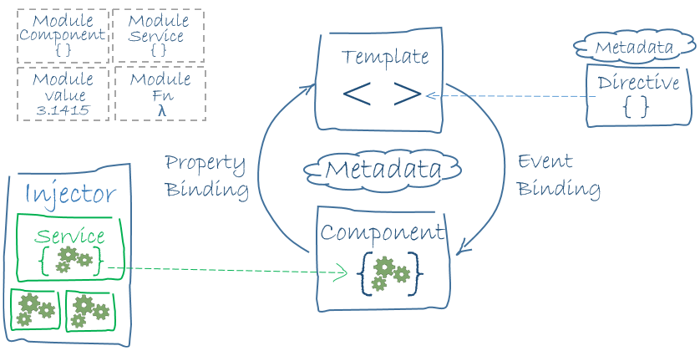
\includegraphics[width=0.8\textwidth]{Chapter1/Figs/angular-overview}
	\caption[Architettura di Angular]{Schema dell'architettura di Angular\cite{angularoverview}}
	\label{fig:angular-overview}
\end{figure}

\section{Attori del sistema}

Dal momento che vi sono più soggetti diversi che accedono alla piattaforma è necessario definire i ruoli dei soggetti coinvolti. Il sistema prevede la gestione di quattro tipi di account --- ognuno con permessi diversi --- e la personalizzazione dell'interfaccia in base all'utente correntemente autenticato. Un account può avere anche più ruoli, ma al momento non ne è previsto l'utilizzo.

\subsection{Azienda}
Rappresenta una (o più) persona fisica responsabile della gestione di un'azienda di cui si fa portavoce.
Deve effettuare l'accesso come un membro esterno dell'ateneo indicando le informazioni della propria azienda e quelle dei suoi amministratori. Inserisce le offerte di tirocinio presso una delle proprie sedi, visualizza le candidature ricevute e approva l'inizio di un tirocinio. Può completare il foglio presenze di un tirocinio in corso nella propria azienda e stamparne la documentazione precompilata al termine. 

\subsection{Professore}
Rappresenta un componente interno all'ateneo che ha il compito di supervisionare le offerte e seguire gli studenti nel percorso.
Deve effettuare l'accesso come un membro dell'ateneo utilizzando l'email istituzionale. Una volta eseguito il login per la prima volta, viene creato un'account il cui ruolo si basa sull'email fornita: se essa termina con \textit{@unive.it} rappresenta un professore, mentre se termina con \textit{@stud.unive.it} rappresenta uno studente. 
Un professore approva le offerte inserite dalle aziende prima che vengano pubblicate, approva e visualizza le richieste di candidatura degli studenti che lo coinvolgono come referente, può completare il foglio presenze di un tirocinio in corso (di cui è referente), e stamparne la documentazione precompilata al termine.

\subsection{Studente}
Rappresenta un componente interno all'ateneo che desidera effettuare un tirocinio in un'azienda.
Deve effettuare l'accesso come un membro dell'ateneo utilizzando l'email istituzionale. Visualizza le offerte di tirocinio pubblicate e propone una candidatura indicando un professore come referente. Può completare il foglio presenze di un suo tirocinio in corso e stamparne la documentazione precompilata al termine.

\subsection{Admin}
Non rappresenta un soggetto fisico, ma bensì una figura che ricopre il ruolo di amministratore dei dati, unico soggetto a non avere restrizioni sulla modifica o la cancellazione di essi. Non ha un'influenza sul processo di gestione dei tirocini in quanto gli altri account formano un ecosistema che si alimenta e gestisce in modo autonomo.
\chapter{Architettura}

Questo capitolo illustra il funzionamento e la struttura delle architetture software, sia per quanto riguarda il \gls{frontend} che il \gls{backend}. Dal momento che entrambe le applicazioni \angular~e \nodejs~operano sugli stessi oggetti, le loro definizioni risiedono in un pacchetto \gls{npm} condiviso che esporta tutte le entità necessarie, in modo da riutilizzare il codice e renderlo facilmente manutenibile. Le principali entità esportate sono:
\begin{itemize}
	\item \textit{User}: rappresenta un utente del sistema con uno specifico ruolo
	\item \textit{Company}: rappresenta un'azienda
	\item \textit{Internship}: rappresenta un'offerta di tirocinio di un'azienda
	\item \textit{InternshipProposal}: rappresenta una proposta di candidatura di uno studente per un tirocinio
\end{itemize}

\section{Architettura lato server}

Il \gls{backend} di \projectName è un'applicazione \nodejs~che si appoggia sul \gls{framework} \expressjs~per l'esposizione di \acrshort{rest} \acrshort{api} che interagiscono con \mongodb~attraverso l'\acrshort{orm} \mongoosejs. \\

\noindent
L'infrastruttura server è divisa in diversi livelli con responsabilità diverse che interagiscono fra loro che verranno discusse nei paragrafi seguenti.

\subsection{Schemas}
Pur utilizzando \mongodb~che è uno schema-less \acrshort{dbms} ho preferito appoggiarmi su un sistema che mi permettesse di validare i dati e la loro struttura. Per fare ciò ho utilizzato \mongoosejs, un \gls{orm} che mi permette di definire la struttura dei documenti nelle collezioni del database, mi fornisce metodi di validazione e manipolazione basati su oggetti.

Gli \textit{schemas} sono la definizione dei documenti delle collezioni del database come previsti da \mongoosejs. Essi contengono la definizione del documento, dei suoi campi e del loro tipo.
% File
\begin{figure}[!h] 
	\centering    
	\lstinputlisting{Chapter2/schema.ts}
	\caption[Esempio di \textit{schema} dell'applicazione \gls{backend}]{Esempio di \textit{schema} dell'applicazione \gls{backend}}
	\label{fig:server-schema}
\end{figure}
Possiamo notare che in figura \ref{fig:server-schema}, all'interno della definizione della struttura del documento, vi sono tre proprietà --- \textit{attendances, internship e status}. Ognuno dei campi ha tipo diverso:
\begin{itemize}
	\item \textit{attendances} è un array di oggetti con una properietà \textit{date} di tipo \textit{Date} obbligatoria
	\item \textit{internship} è una referenza di un altro schema (Internship), che verrà popolato automaticamente in fase di lettura (effettua un \gls{sqljoin} in automatico con il plugin \acrshort{npm} `mongoose-autopopulate`)
	\item \textit{status} è semplice numero
\end{itemize}
Nel caso l'applicazione cerchi di salvare un oggetto che non rispetti i vincoli imposti dallo \textit{schema} viene sollevata un'eccezione che impedisce di rendere inconsistente il database.

\subsection{Repositories}
I \textit{repositories} sono classi legate ad uno specifico oggetto che esportano operazioni su di esso. Interrogano uno o più \textit{schemas} per leggere, scrivere o aggregare dati, e contengono solamente la logica di accesso ai dati, senza nessuna logica di business (ad esempio il controllo dei permessi). Tutti i \textit{repositories} dervano dal \textit{BaseRepository} che esporta le operazioni di base --- \gls{crud} --- oltre che un metodo per eseguire query personalizzate.
% File
\begin{figure}[!h] 
	\centering    
	\lstinputlisting{Chapter2/repository.ts}
	\caption[Esempio di \textit{Repository}]{Esempio di \textit{repository} dell'applicazione \gls{backend}}
	\label{fig:server-repository}
\end{figure}
Ogni \textit{repository} può esporre ulteriori metodi personalizzati ed eventualmente accedere e ad altri \textit{repositories} iniettati dal sistema di \acrfull{di}. Il sistema di \acrshort{di} adottato dal sistema si basa sul pacchetto \acrshort{npm} `inversisy`, che fornisce anche un modo di aggirare le dipendenze circolari (ad esempio tra due \textit{repositories}) tramite un meccanismo di \textit{lazy-inject}.


\subsection{Controllers}
\label{server:controllers}
I \textit{controllers} espongono su architettura \acrshort{rest} \acrshort{api} un metodo di \expressjs~ che internamente utilizza le operazioni dei \textit{repositories}. Anche i \textit{controllers} sono legati ad un unica entità e dervano da un \textit{BaseController} che di default espone i metodi per le operazioni di \acrshort{crud} dell'entità. Tutti i metodi esposti ritornano il risultato wrappato all'interno di un oggetto, \textit{ApiResponseDto}, che contiene anche informazioni aggiuntive, come lo stato \acrshort{http} ed eventuali errori.
%
I \textit{controllers} sono responsabili di gestire l'autenticazione dell'utente e le eventuiali eccezioni sollevate dai \textit{repositories}. Ogni \textit{controller} può esporre metodi che richiedono ruoli diversi, quindi ogni metodo definisce tramite uno \textit{\hyperref[server:scopes]{autentication middleware}} quale siano gli utenti abilitati ad eseguire quel metodo e in caso negativo ritorna un errore di autenticazione.

\begin{figure}[H] 
	\centering    
	\lstinputlisting{Chapter2/controller1.ts}
	\caption[Esempio di registrazione di un metodo \expressjs~in un \textit{Controller}]{Esempio di registrazione di un metodo \expressjs~in un \textit{Controller}}
	\label{fig:server-controller-1}
\end{figure}

\noindent
Come possiamo notare in figura \ref{fig:server-controller-1} il \textit{controller} sta registrando una route di \expressjs~il cui  secondo parametro è un array. Queso array contiene un insieme di \textit{middleware} che \expressjs~si occuperà di invocare prima di eseguire il codice all'interno della \gls{callback}. Il \textit{middleware}, in questo caso la funzione \textit{ownInternshipProposal}, verifica che l'utente che ha effettuato la chiamata sia effettivamente un soggetto (azienda, professore o studente) della proposta di tirocinio di cui vuole aggiornare lo stato. In caso negativo rifiuta la richiesta con un errore e la termina. L'autenticazione del sistema verrà discussa in dettaglio nel capitolo \textit{\ref{chap:api} - \nameref{chap:api}}.

\subsection{Bootstrap}

L'avvio dell'applicazione avviene nel file \textit{server.ts}, che si preoccupa di registrare tutti i \textit{repositories} nel sistema di \acrlong{di} e infine di rispolvere i \textit{controllers}.
\begin{figure}[H] 
	\centering    
	\lstinputlisting{Chapter2/server.ts}
	\caption[Estratto di \textit{Server.ts}, bootstrap del \gls{backend}]{Estratto di \textit{Server.ts}, bootstrap del \gls{backend}}
	\label{fig:server-bootstrap}
\end{figure}

\noindent
L'applicazione si preoccupa anche di connettersi al database \mongodb~e registrare nel container l'istanza dell'applicazione in modo sia accessibile dove necessario. Definisce inoltre un \textit{middleware} per catturare eventuali eccezioni non gestite dai \textit{controllers}.

\pagebreak
\section{Archietettura lato client}

Il \gls{frontend} di \projectName~è un'applicazione \angular~(v6) composta da diversi moduli (\nameref{chap:ngmodules}). Vi sono due moduli principali, uno che contiene le pagine che può visualizzare un utente non autenticato (\textit{NoAuthModule}) e uno che contiene le pagine visibili agli utenti autenticati (\textit{AuthModule}). Il modulo per gli utenti non autenticati viene caricato per primo, mentre il modulo che contiene le pagine protette viene caricato con la tecnica del \textit{lazy-loading} solamente una volta effettuato il login. Esiste poi un altro macro modulo, \textit{SharedModule}, che contiene dipendenze utilizzare in entrambi gli altri due moduli e che viene infatti importato in essi.

\subsection{Moduli e divisione delle responsabilità}
\label{client:modules}
\subsubsection{SharedModule}
\label{client:shared-module}
Contiene le dipendenze, i \textit{components}, le \textit{pipes} e le \textit{directives} utilizzate negli altri moduli. Viene importato sia in \textit{NoAuthModule} che in \textit{AuthModule}.

\subsubsection{NoAuthModule}
\label{client:no-auth-module}
Contiene la pagine che solo un utente non autenticato può raggiungere, ovvero \textit{login} di un utente e \textit{registrazione} di un'azienda. Una volta effettuato il login, il \textit{router} carica il modulo \textit{AuthModule} che contiene invece tutte le pagine protette e fintanto che l'utente non effettua il \textit{logout} non può più raggiungere le pagine in \textit{NoAuthModule}.


\subsubsection{AuthModule}
\label{client:auth-module}
Contiene la pagine che solo un utente autenticato può raggiungere, ovvero il cuore dell'applicazione. Data la sua dimensione questo modulo contiene degli altri sotto moduli:
\begin{itemize}
	\item \textit{UserModule}: contiene la parte di gestione dell'account di un utente, con la possibilità di modificarlo
	\item \textit{Internship}: contiene la parte di gestione dei tirocini (aggiunta, modifica, approvazione, dettaglio, candidatura)
	\item \textit{InternshipProposal}: contiene la parte di gestione dei tirocini (modifica, approvazione, dettaglio, tracciamento)
	\item \textit{Shared}: contiene i componenti comuni a questi sotto moduli (header, footer e sidebar)
\end{itemize}


\subsection{Servizi e recupero dei dati}
\label{client:services}
I moduli visti poco sopra contengono i componenti responsabili della visualizzazione dei dati, che tuttavia non si preoccupano di recuperare in autonomia. Essi si affidano infatti ad uno strato di servizi che interagiscono con il \gls{backend} dell'applicazione, i \textit{services}.
I \textit{services} di \angular~seguono lo standard del \gls{backend}, ovvero ognuno di essi si preoccupa di gestire una sola entità.
 \begin{figure}[!h] 
 	\centering    
 	\lstinputlisting{Chapter2/service.ts}
 	\caption[Esempio di \textit{service} \gls{frontend}]{Esempio di \textit{service} \gls{frontend}}
 	\label{fig:client-service}
 \end{figure}
All'interno dei componenti che contengono il \textit{template} verranno iniettati uno o più \textit{services} che permetteranno di recuperare i dati da visualizzare.

 \subsection{Supporto multi lingua}
 La gestione della localizzazione dell'app è gestita tramite il pacchetto \acrshort{npm} \textit{ngx-translate}, che fornisce dei componenti per la traduzione delle stringhe nei \textit{template} dei \textit{components} e nei relativi \textit{view-model}. Le traduzioni sono salvate in un file \acrshort{json}
 \begin{figure}[!h] 
	\centering    
	\lstinputlisting{Chapter2/globalization.json}
	\caption[Estratto del file di globalizzazione \gls{frontend}]{Estratto del file di globalizzazione \gls{frontend}}
	\label{fig:client-globalization}
\end{figure}
ed è possibile recuperare in differenti modi:
\begin{itemize}
	\item \textit{Pipe}: da utilizzare nel \textit{template} quando ci sono espressioni da valutare
	\item \textit{Directive}: da utilizzare nel \textit{template} quando la stringa da tradurre è cablata
	\item \textit{Service}: da utilizzare nel \textit{view-model} dei \textit{components}
\end{itemize}
 \begin{figure}[!h] 
	\centering    
	\lstinputlisting{Chapter2/globalization.ts}
	\caption[Localizzare un \textit{component} con \textit{ngx-translate}]{Localizzare un \textit{component} con \textit{ngx-translate}}
	\label{fig:client-ngxtranslate}
\end{figure}
Un servizio registrato al \textit{bootstrap} dell'applicazione si preoccupa di leggere la lingua corrente e caricare il file di traduzione relativo, oppure uno di \textit{fallback}.
\chapter{Casi d'uso e workflow}

\section{Casi d'uso}
And now I begin my third chapter here 

\subsection{Creazione di un'utente}

Deve essere possibile creare (ovvero registrare) un nuovo utente nella piattaforma. 

\subsection{UC-2: Login di un'utente}
\dots and some more \dots

\chapter{API}

\section{Autenticazione}

Express middleware, auth controller

\subsection{Server side}

Utilizzo JWT per gestire lo stato del sistema

\subsection{Client side}

Utilizzo JWT per gestire lo stato del sistema

\section{Endpoints}

\subsection{Controller base}
Descrizione controller base

\begin{table}[h]
    \ttfamily
    \caption{Endpoint rest API}
    \centering
    \label{table:good_table}
    \begin{tabular}{l c c c c}
    
    
    URL  & Metodo & Parametri  & Risposta  \\ 
    \midrule
    /api/internship & GET &  & ApiResponseDto<Array<Internship>>   \\
    
    I1LL & 7.48 & 0.56 & 8.7  \\
    
    I2MD & 3.99 & 0.63 & 4.2 \\
    
    I2LL & 6.81 & 0.02 & 6.66 \\
    
    CMD & 13.47 & 0.09 & 10.55 \\
    
    CBL & 11.88 & 0.05 & 13.11\\ 
    \bottomrule
    \end{tabular}
    \end{table}

\subsection{Internships}
Metodi custom

\subsection{InternshipProposals}
Metodi custom

\subsection{Roles}
Metodi custom

\subsection{Users}
Metodi custom

\subsection{Companies}
Metodi custom

\subsection{Auth}
Metodi custom

\chapter{Conclusioni}

L'applicazione, sebbene soddisfi i casi d'uso previsti, è da considerarsi come una versione non ancora in grado di ricoprire tutti gli scenari realmente esistenti nel processo di gestione dei tirocini. Quello che potrebbe completare \projectName~è l'integrazione dell'autenticazione con il sistema federato dell'ateneo e l'aggiunta del ruolo utente "Garante"  --- che potrebbe convergere con il ruolo di professore~--- che si occupa di accertare che il tirocinio richiesto da uno studente possa permettere il riconoscimento di crediti formativi. In questo momento, infatti, la candidatura ad un tirocinio è da considerarsi come extra-curricolare. 
%
Per permettere il riconoscimento di crediti formativi è necessario che l'azienda sia convenzionata con l'ateneo e che il contenuto del tirocinio sia valido e inerente al percorso di studi. Per questo si potrebbe pensare di creare una sezione dell'applicazione che permetta di convenzionare le aziende interessate, e infine di consentire al professore di verificare che il piano dell'azienda proposto per il tirocinio sia sufficiente al riconoscimento dei crediti richiesti dallo studente.

\section{Sviluppi futuri e nuove integrazioni}
I possibili sviluppi futuri dell'applicazione potrebbero dunque coinvolgere:
\begin{itemize}
	\item la gestione di stage anche curriculari, permettendo il riconoscimento dei crediti formativi universitari (CFU)
	\item l'autenticazione mediante il sistema federato dell'ateneo, permettendo un controllo degli utenti più restrittivo
	\item la possibilità di convenzionare le aziende online, favorendo il numero di imprese che interagiscono con l'ateneo
\end{itemize}



% ********************************** Bibliography ******************************
\begin{spacing}{0.9}

\bibliographystyle{plainnat} % use this to have URLs listed in References
\cleardoublepage
\bibliography{References/references} % Path to your References.bib file


\end{spacing}

% ********************************** Appendices ********************************

\begin{appendices} % Using appendices environment for more functunality

%%!TEX root = ../thesis.tex
% ******************************* Thesis Appendix A ****************************
\chapter{How to install \LaTeX} 

\section*{Windows OS}

\subsection*{TeXLive package - full version}
\begin{enumerate}
\item	Download the TeXLive ISO (2.2GB) from\\
\href{https://www.tug.org/texlive/}{https://www.tug.org/texlive/}
\item	Download WinCDEmu (if you don't have a virtual drive) from \\
\href{http://wincdemu.sysprogs.org/download/}
{http://wincdemu.sysprogs.org/download/}
\item	To install Windows CD Emulator follow the instructions at\\
\href{http://wincdemu.sysprogs.org/tutorials/install/}
{http://wincdemu.sysprogs.org/tutorials/install/}
\item	Right click the iso and mount it using the WinCDEmu as shown in \\
\href{http://wincdemu.sysprogs.org/tutorials/mount/}{
http://wincdemu.sysprogs.org/tutorials/mount/}
\item	Open your virtual drive and run setup.pl
\end{enumerate}

or

\subsection*{Basic MikTeX - \TeX~ distribution}
\begin{enumerate}
\item	Download Basic-MiK\TeX (32bit or 64bit) from\\
\href{http://miktex.org/download}{http://miktex.org/download}
\item	Run the installer 
\item	To add a new package go to Start >> All Programs >> MikTex >> Maintenance (Admin) and choose Package Manager
\item	Select or search for packages to install
\end{enumerate}

\subsection*{TexStudio - \TeX~ editor}
\begin{enumerate}
\item	Download TexStudio from\\
\href{http://texstudio.sourceforge.net/\#downloads}
{http://texstudio.sourceforge.net/\#downloads} 
\item	Run the installer
\end{enumerate}

\section*{Mac OS X}
\subsection*{MacTeX - \TeX~ distribution}
\begin{enumerate}
\item	Download the file from\\
\href{https://www.tug.org/mactex/}{https://www.tug.org/mactex/}
\item	Extract and double click to run the installer. It does the entire configuration, sit back and relax.
\end{enumerate}

\subsection*{TexStudio - \TeX~ editor}
\begin{enumerate}
\item	Download TexStudio from\\
\href{http://texstudio.sourceforge.net/\#downloads}
{http://texstudio.sourceforge.net/\#downloads} 
\item	Extract and Start
\end{enumerate}


\section*{Unix/Linux}
\subsection*{TeXLive - \TeX~ distribution}
\subsubsection*{Getting the distribution:}
\begin{enumerate}
\item	TexLive can be downloaded from\\
\href{http://www.tug.org/texlive/acquire-netinstall.html}
{http://www.tug.org/texlive/acquire-netinstall.html}.
\item	TexLive is provided by most operating system you can use (rpm,apt-get or yum) to get TexLive distributions
\end{enumerate}

\subsubsection*{Installation}
\begin{enumerate}
\item	Mount the ISO file in the mnt directory
\begin{verbatim}
mount -t iso9660 -o ro,loop,noauto /your/texlive####.iso /mnt
\end{verbatim}

\item	Install wget on your OS (use rpm, apt-get or yum install)
\item	Run the installer script install-tl.
\begin{verbatim}
	cd /your/download/directory
	./install-tl
\end{verbatim}
\item	Enter command `i' for installation

\item	Post-Installation configuration:\\
\href{http://www.tug.org/texlive/doc/texlive-en/texlive-en.html\#x1-320003.4.1}
{http://www.tug.org/texlive/doc/texlive-en/texlive-en.html\#x1-320003.4.1} 
\item	Set the path for the directory of TexLive binaries in your .bashrc file
\end{enumerate}

\subsubsection*{For 32bit OS}
For Bourne-compatible shells such as bash, and using Intel x86 GNU/Linux and a default directory setup as an example, the file to edit might be \begin{verbatim}
edit $~/.bashrc file and add following lines
PATH=/usr/local/texlive/2011/bin/i386-linux:$PATH; 
export PATH 
MANPATH=/usr/local/texlive/2011/texmf/doc/man:$MANPATH;
export MANPATH 
INFOPATH=/usr/local/texlive/2011/texmf/doc/info:$INFOPATH;
export INFOPATH
\end{verbatim}
\subsubsection*{For 64bit OS}
\begin{verbatim}
edit $~/.bashrc file and add following lines
PATH=/usr/local/texlive/2011/bin/x86_64-linux:$PATH;
export PATH 
MANPATH=/usr/local/texlive/2011/texmf/doc/man:$MANPATH;
export MANPATH 
INFOPATH=/usr/local/texlive/2011/texmf/doc/info:$INFOPATH;
export INFOPATH

\end{verbatim}



%\subsection{Installing directly using Linux packages} 
\subsubsection*{Fedora/RedHat/CentOS:}
\begin{verbatim} 
sudo yum install texlive 
sudo yum install psutils 
\end{verbatim}


\subsubsection*{SUSE:}
\begin{verbatim}
sudo zypper install texlive
\end{verbatim}


\subsubsection*{Debian/Ubuntu:}
\begin{verbatim} 
sudo apt-get install texlive texlive-latex-extra 
sudo apt-get install psutils
\end{verbatim}


\end{appendices}

% *************************************** Index *******************************
\glsaddall
\printglossary[type=\acronymtype,title=Arconimi,toctitle=Acronimi] % prints just the list of acronyms
\printglossary % if no option is supplied the default glossary is printed.
\end{document}
